\begin{figure}[ht]
    \centering
        \begin{subfigure}[t]{0.32\textwidth}
    	\centering
       	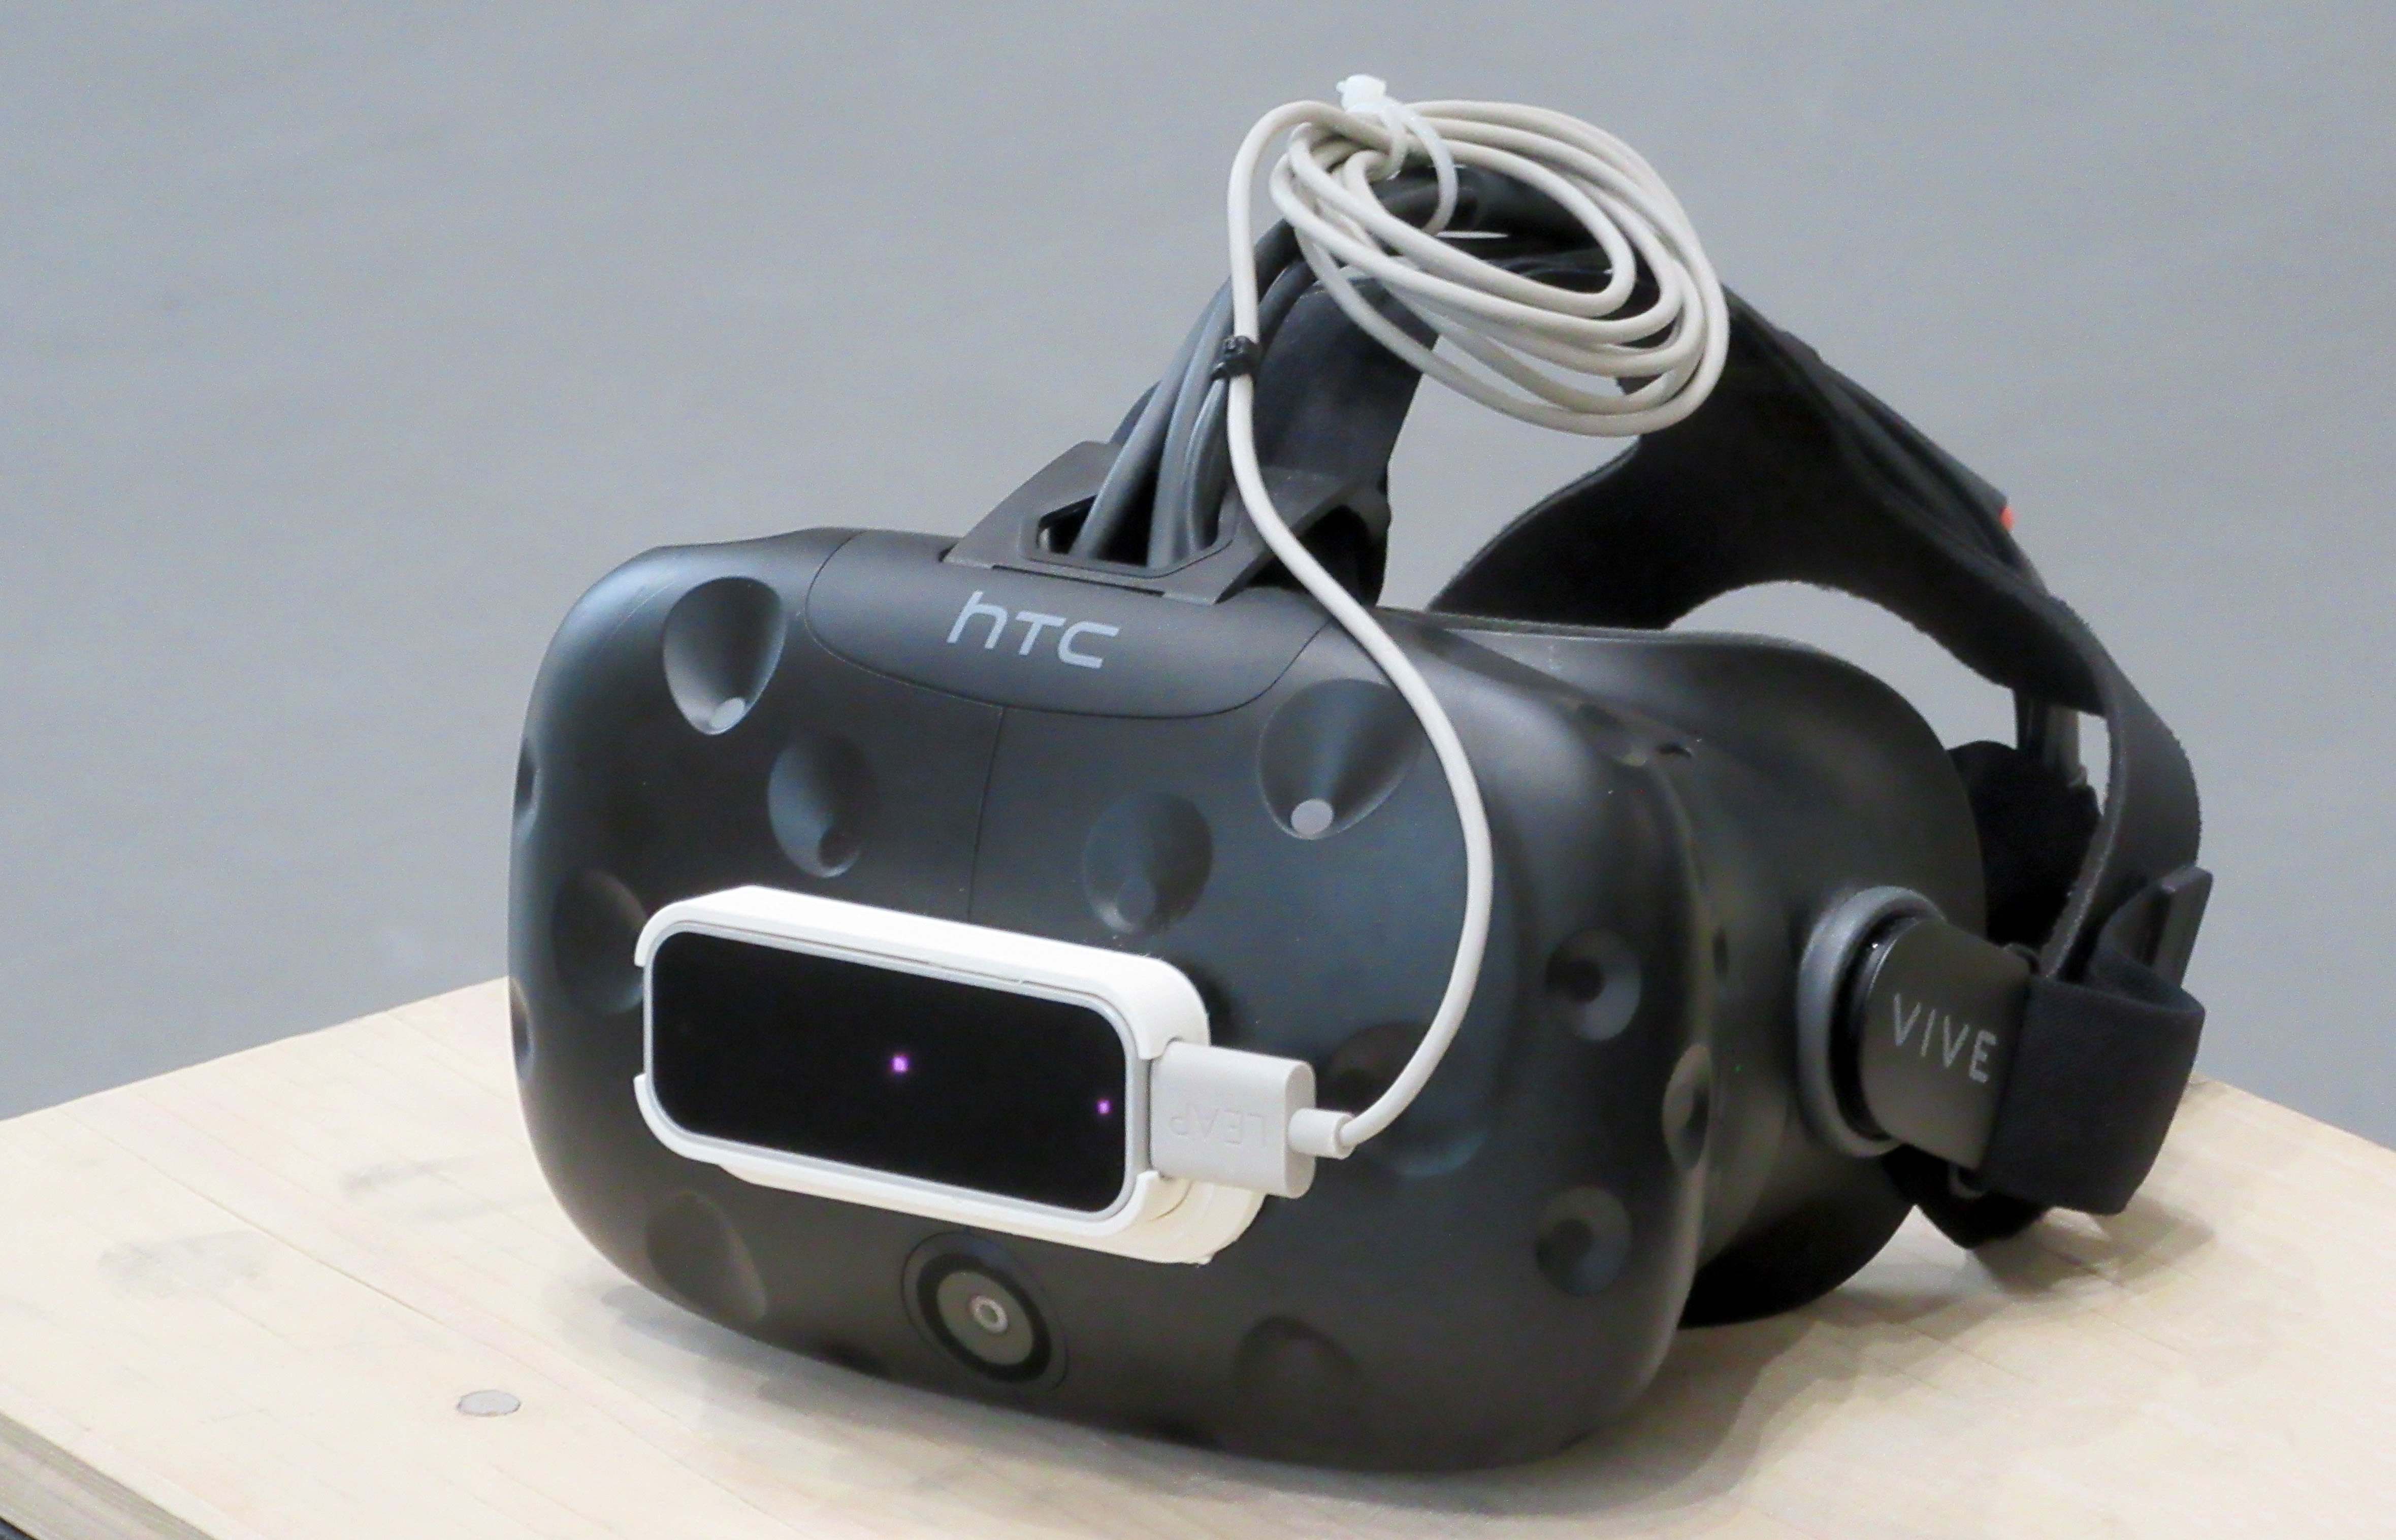
\includegraphics[width=\textwidth]{include/images/leap-motion-overlay-setup.jpg}
    	\caption{The Leap Motion sensor mounted on VIVE headset}
    	\label{fig:leap-motion-setup}
    \end{subfigure}
    \hfill
    \begin{subfigure}[t]{0.32\textwidth}
        \centering
       	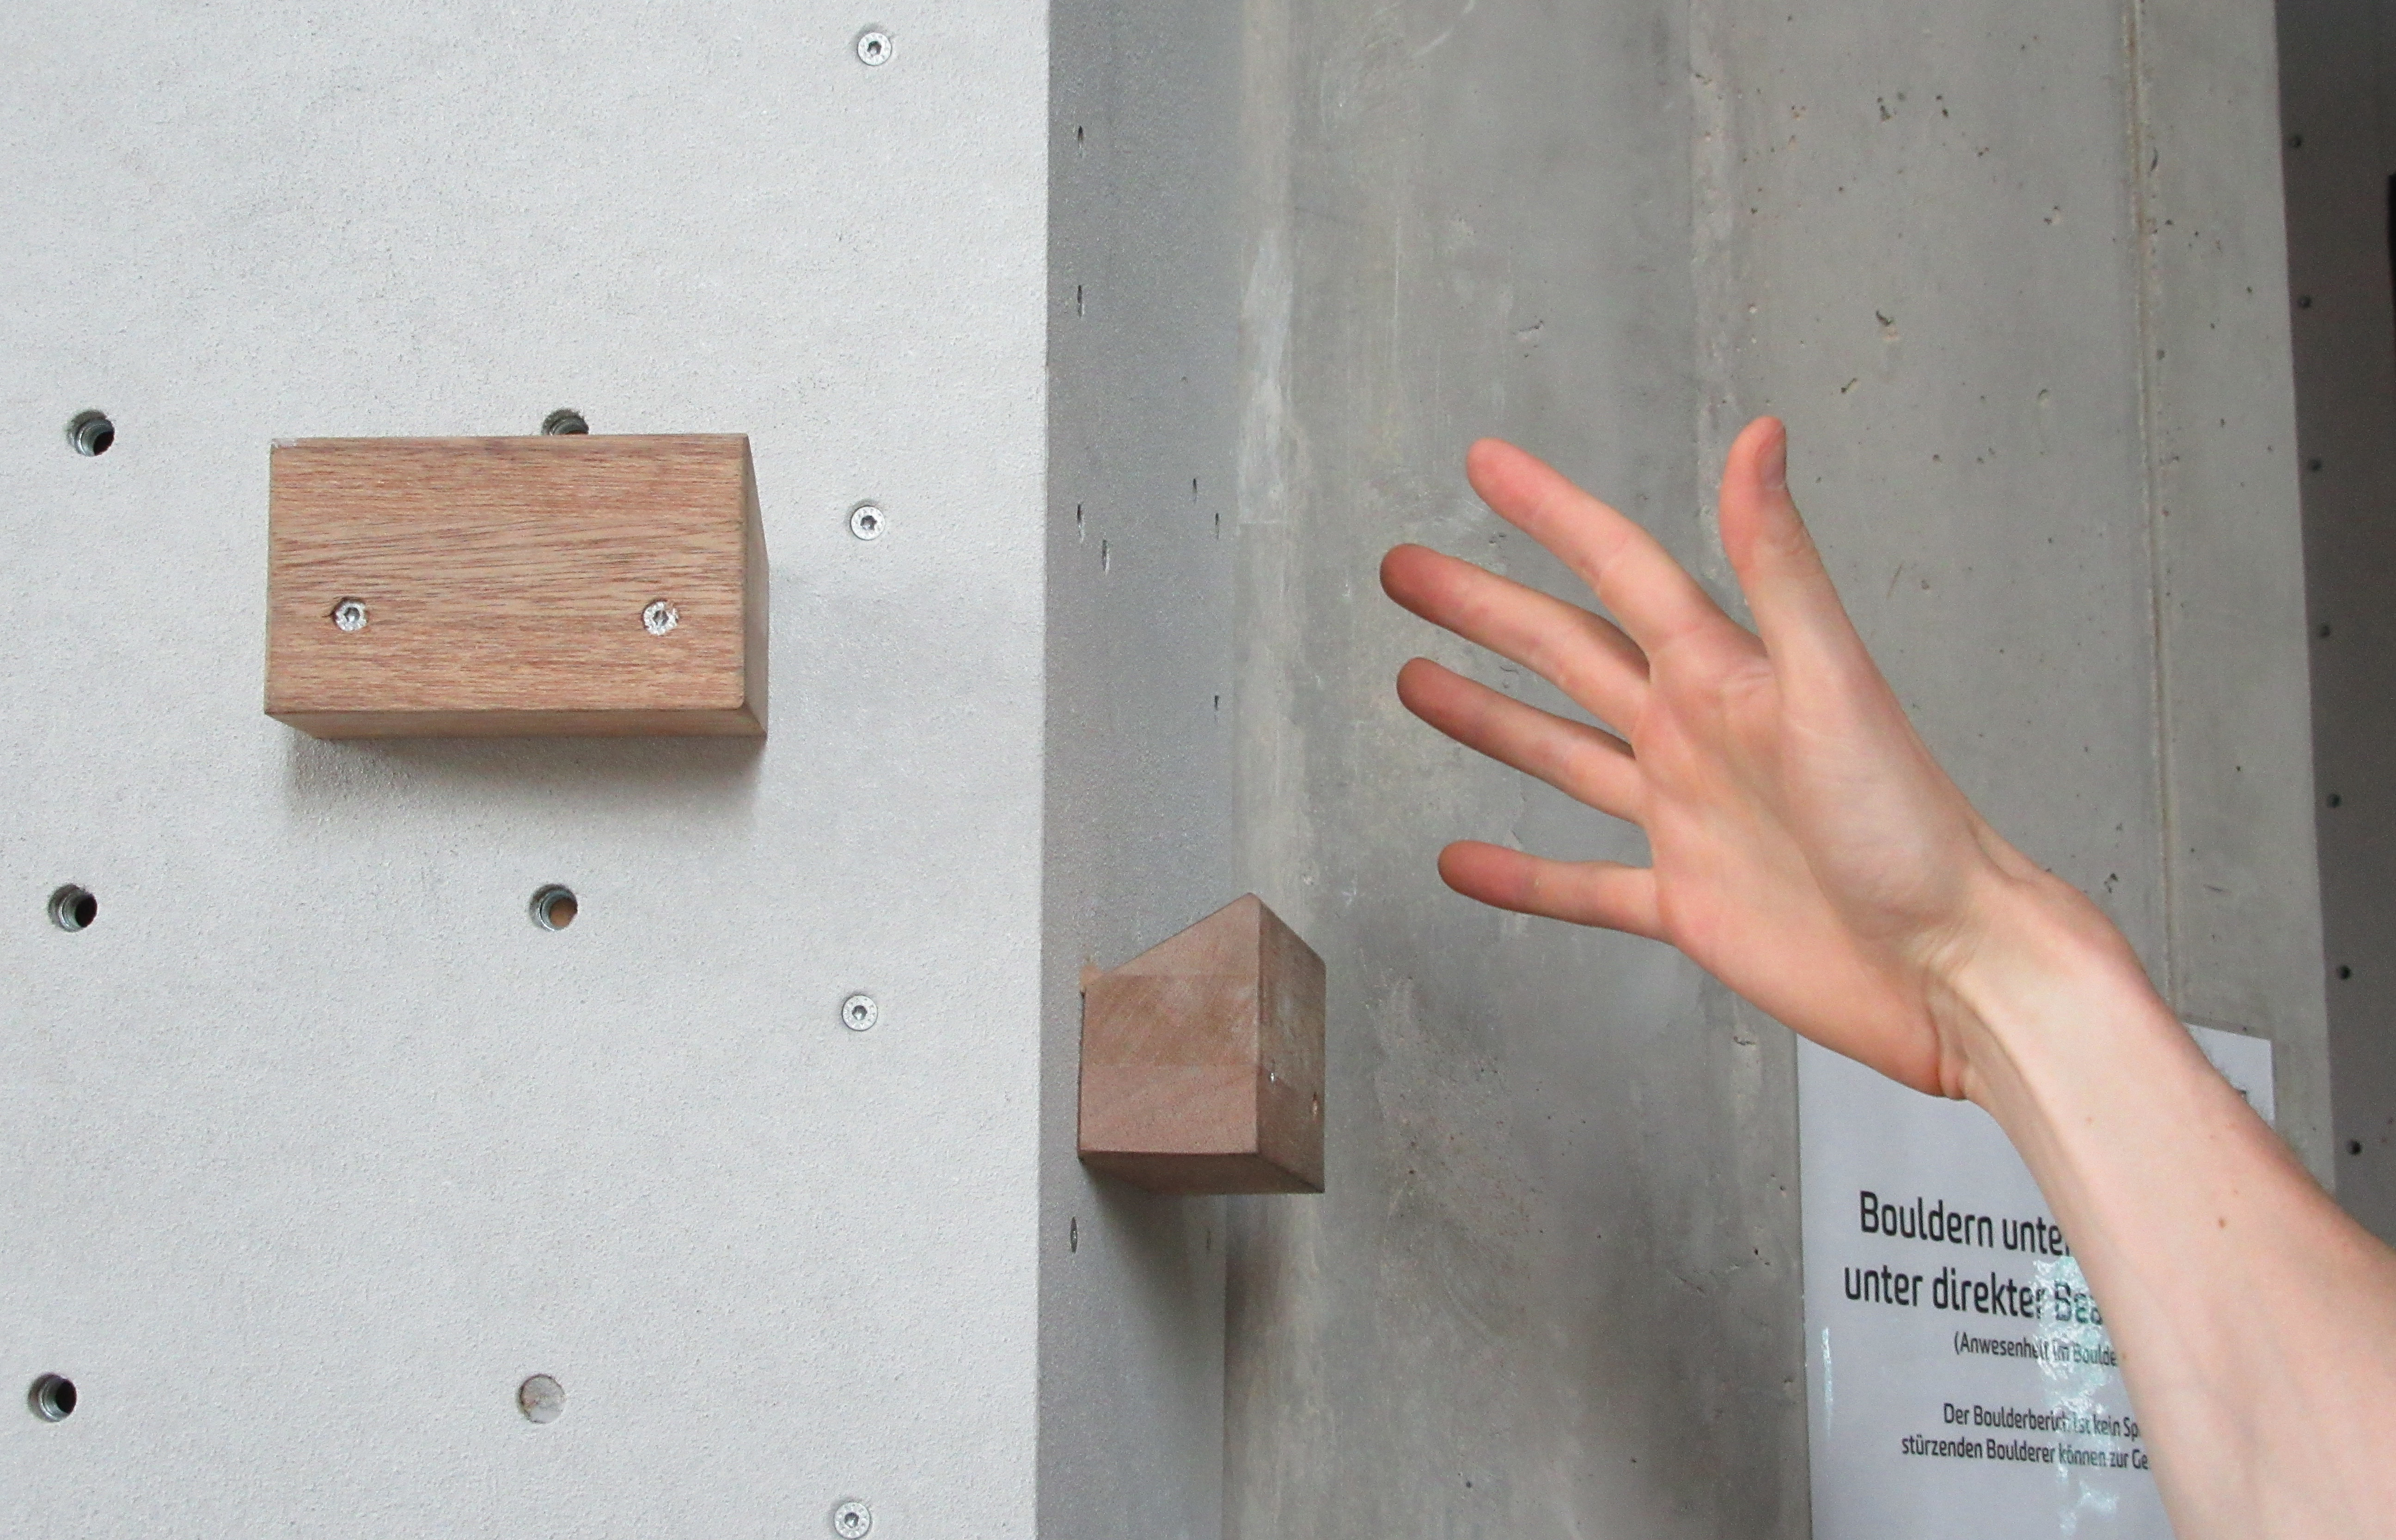
\includegraphics[width=\textwidth]{include/images/leap-motion-overlay-photo.jpg}
        \caption{Photo of a right hand over a handhold}
        \label{fig:leap-motion-overlay-photo}
    \end{subfigure}
    \hfill
	\begin{subfigure}[t]{0.32\textwidth}
		\centering
		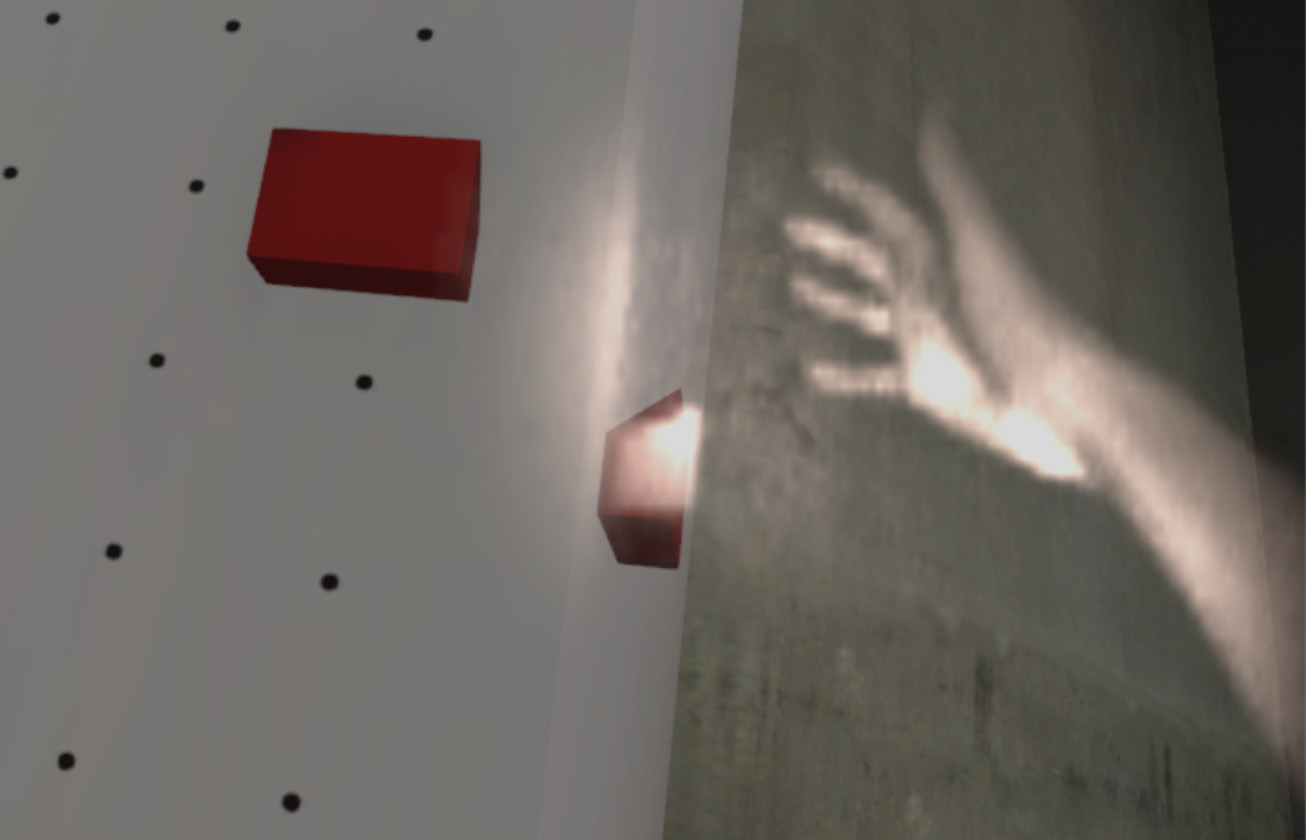
\includegraphics[width=\textwidth]{include/images/leap-motion-overlay-result.jpg}
		\caption{Screenshot of the resulting, masked infrared overlay}
		\label{fig:leap-motion-overlay-result}
	\end{subfigure}
	\captionsetup{subrefformat=parens}
    \caption[Leap Motion hand tracking]{Leap Motion hand overlay created from the infrared image provided by the sensor \subref{fig:leap-motion-setup} masked with a blurred image of the rendered hand models, which makes objects near the hands, such as the hand holds, visible as well \subref{fig:leap-motion-overlay-result}}
    \label{fig:leap-motion-overlay}
\end{figure}